% --------------------------------------------------------------------------- %
% Created with Brian Amberg's LaTeX Poster Template. Please refer for the     %
% attached README.md file for the details how to compile with `pdflatex`.     %
% --------------------------------------------------------------------------- %
\documentclass[paperwidth=80cm,paperheight=105cm,fontscale=0.35,margin=10px]{baposter}

\usepackage{relsize}		% For \smaller
\usepackage{url}			% For \url
\usepackage{epstopdf}	% Included EPS files automatically converted to PDF to include with pdflatex
\usetikzlibrary{fit,positioning,calc}
\usepackage{amsmath}
\usepackage{amssymb}
\usepackage{tcolorbox}
\usepackage{picture}
\usepackage{relsize}
\usepackage{tikz}


%\usepackage[utf8]{inputenc}

%%% Global Settings %%%%%%%%%%%%%%%%%%%%%%%%%%%%%%%%%%%%%%%%%%%%%%%%%%%%%%%%%%%

\graphicspath{{pix/}}	% Root directory of the pictures 
\tracingstats=2			% Enabled LaTeX logging with conditionals

%%% Color Definitions %%%%%%%%%%%%%%%%%%%%%%%%%%%%%%%%%%%%%%%%%%%%%%%%%%%%%%%%%

\definecolor{bordercol}{RGB}{40,40,40}
\definecolor{original1}{RGB}{188,209,176} 
\definecolor{lightbluegreen1}{RGB}{200,236,210} 
\definecolor{darkbluegreen1}{RGB}{16,82,71}
\definecolor{lightorange1}{RGB}{255,255,204} 
\definecolor{darkorange1}{RGB}{174,62,7} 
\definecolor{darkred1}{RGB}{60,2,2}
\definecolor{darkpurple1}{RGB}{129,0,39}
\definecolor{original2}{RGB}{127,158,153}
\definecolor{lightbluegreen2}{RGB}{134,193,173} 
\definecolor{darkbluegreen2}{RGB}{23,131,113} 
\definecolor{lightorange2}{RGB}{246,194,19} 
\definecolor{darkorange2}{RGB}{230,83,9} 
\definecolor{darkred2}{RGB}{190,0,0} 
\definecolor{darkpurple2}{RGB}{205,0,61}
\definecolor{headerfontcol}{RGB}{255,255,255}
\definecolor{boxcolor}{RGB}{255,249,225}
\definecolor{boxcolor2}{RGB}{255,249,225}
%\definecolor{bkgcol}{RGB}{230,250,230}%lightgreenblue
\definecolor{bkgcol}{RGB}{255,255,255}
\definecolor{phenixgreen}{RGB}{50,205,50}
\definecolor{phenixdarkgreen}{RGB}{45,170,45}
\definecolor{qm2}{RGB}{206, 230, 253}
\definecolor{qm1}{RGB}{252, 235, 233}
\definecolor{bl1}{RGB}{33, 1, 178}
\definecolor{bl2}{RGB}{89, 52, 254}
\definecolor{rd2}{RGB}{131, 103, 254}
\definecolor{rd1}{RGB}{107, 51, 255}
\definecolor{ab}{RGB}{102, 0, 0}

%%%%%%%%%%%%%%%%%%%%%%%%%%%%%%%%%%%%%%%%%%%%%%%%%%%%%%%%%%%%%%%%%%%%%%%%%%%%%%%%
%%% Utility functions %%%%%%%%%%%%%%%%%%%%%%%%%%%%%%%%%%%%%%%%%%%%%%%%%%%%%%%%%%

%%% Save space in lists. Use this after the opening of the list %%%%%%%%%%%%%%%%
\newcommand*{\bfrac}[2]{\genfrac{}{}{0pt}{}{#1}{#2}}

\newcommand{\compresslist}{
	\setlength{\itemsep}{1pt}
	\setlength{\parskip}{0pt}
	\setlength{\parsep}{0pt}
}
\newcommand{\cimg}[2]{
\begin{center}
  \setlength{\abovedisplayskip}{0pt}
\includegraphics[width=#2\linewidth]{#1}
\end{center}
}

\newenvironment{tightitemize}{
  \setlength{\leftmargini}{10pt}
\begin{itemize}
  \setlength{\leftmargin}{0pt}
  \setlength{\parskip}{0pt}
  \setlength{\parsep}{0pt}
  \setlength{\itemsep}{0pt}
}{\end{itemize}}

\newenvironment{tightequation}{
  \setlength{\leftmargini}{0pt}
\begin{displaymath}
  \setlength{\leftmargin}{0pt}
  \setlength{\parskip}{0pt}
  \setlength{\parsep}{0pt}
  \setlength{\itemsep}{0pt}
  \setlength{\abovedisplayskip}{1.8pt}
  \setlength{\belowdisplayskip}{2.5pt}
}{\end{displaymath}}

\usepackage[pscoord]{eso-pic}% The zero point of the coordinate systemis the lower left corner of the page (the default).

\newcommand{\placetextbox}[3]{% \placetextbox{<horizontal pos>}{<vertical pos>}{<stuff>}
  \setbox0=\hbox{#3}% Put <stuff> in a box
  \AddToShipoutPictureFG*{% Add <stuff> to current page foreground
    \put(\LenToUnit{#1\paperwidth},\LenToUnit{#2\paperheight}){\vtop{{\null}\makebox[0pt][c]{#3}}}%
  }%
}%



%%%%%%%%%%%%%%%%%%%%%%%%%%%%%%%%%%%%%%%%%%%%%%%%%%%%%%%%%%%%%%%%%%%%%%%%%%%%%%%
%%% Document Start %%%%%%%%%%%%%%%%%%%%%%%%%%%%%%%%%%%%%%%%%%%%%%%%%%%%%%%%%%%%
%%%%%%%%%%%%%%%%%%%%%%%%%%%%%%%%%%%%%%%%%%%%%%%%%%%%%%%%%%%%%%%%%%%%%%%%%%%%%%%

\begin{document}

\typeout{Poster rendering started}

%%% Setting Background Image %%%%%%%%%%%%%%%%%%%%%%%%%%%%%%%%%%%%%%%%%%%%%%%%%%
%\background{
%\begin{tikzpicture}[remember picture,overlay]%
%      \draw (current page.north west)+(-2em,2em) node[anchor=north west]
%      {\includegraphics[width=1.1\textwidth]{screenshot38_v3}};
%      \end{tikzpicture}%
%}

%%% General Poster Settings %%%%%%%%%%%%%%%%%%%%%%%%%%%%%%%%%%%%%%%%%%%%%%%%%%%
%%%%%% Eye Catcher, Title, Authors and University Images %%%%%%%%%%%%%%%%%%%%%%
\begin{poster}{
	grid=false,
	% Option is left on true though the eyecatcher is not used. The reason is
	% that we have a bit nicer looking title and author formatting in the headercol
	% this way
	eyecatcher=true, 
	borderColor=bordercol,
	headerColorOne=lightorange1,
	headerColorTwo=lightorange2,
	headerFontColor=headerfontcol,
	% Only simple background color used, no shading, so boxColorTwo isn't necessary
	boxColorOne=white,%boxcolor,
	boxColorTwo=white,%boxcolor2,
	headershape=roundedright,
	headerfont=\large\sf\bf,
	textborder=rectangle,
	bgColorOne=qm1,%bkgcol,
	bgColorTwo=qm2,%phenixdarkgreen,
	background=shadeTB,%shade-tb,%user,
	headerborder=open,
    boxshade=plain,
    %boxopacity=.55
}
%%% Eye Cacther %%%%%%%%%%%%%%%%%%%%%%%%%%%%%%%%%%%%%%%%%%%%%%%%%%%%%%%%%%%%%%%
{
\begin{minipage}{0.2\textwidth}%\baposter@titleimage@textwidth
  \begin{center}%
    
\includegraphics[height=6.5em]{figs/qmlogo}\\
     \vspace{-0.01\textheight}
    
\includegraphics[height=4.5em]{figs/logo_100}
         \vspace{-0.02\textheight}
  \end{center}%
\end{minipage}
}
%%% Title %%%%%%%%%%%%%%%%%%%%%%%%%%%%%%%%%%%%%%%%%%%%%%%%%%%%%%%%%%%%%%%%%%%%%
{\sf\bf \huge
\vspace{-6pt}
PHENIX results on Levy analysis of\\ %{\fontsize{28}{24}\selectfont 
three\vspace{-2pt}
 particle \\Bose-Einstein correlation functions\vspace{-0.01\textheight}
}
%%% Authors %%%%%%%%%%%%%%%%%%%%%%%%%%%%%%%%%%%%%%%%%%%%%%%%%%%%%%%%%%%%%%%%%%%
{
\noindent \rule{0.9\textwidth}{1.2pt}\\ \vspace{-0.005\textheight}
	{\smaller Attila Bagoly (E�tv�s University, Budapest) for the PHENIX Collaboration}\vspace{-0.01\textheight}

}
%%%University Logo
{
\begin{minipage}{0.2\textwidth}%\baposter@titleimage@textwidth
  \begin{center}%
	
\includegraphics[height=5em]{figs/BNL2}\\
	     \vspace{-0.012\textheight}
		
\includegraphics[height=6em]{figs/ELTE}
			     \vspace{-0.02\textheight}

  \end{center}
\end{minipage}
\vspace{-0.1\textheight}
}

\headerbox{The PHENIX experiment at RHIC}{name=aaa,column=0,headerFontColor=black}{
\begin{center}
\vspace{-2pt}
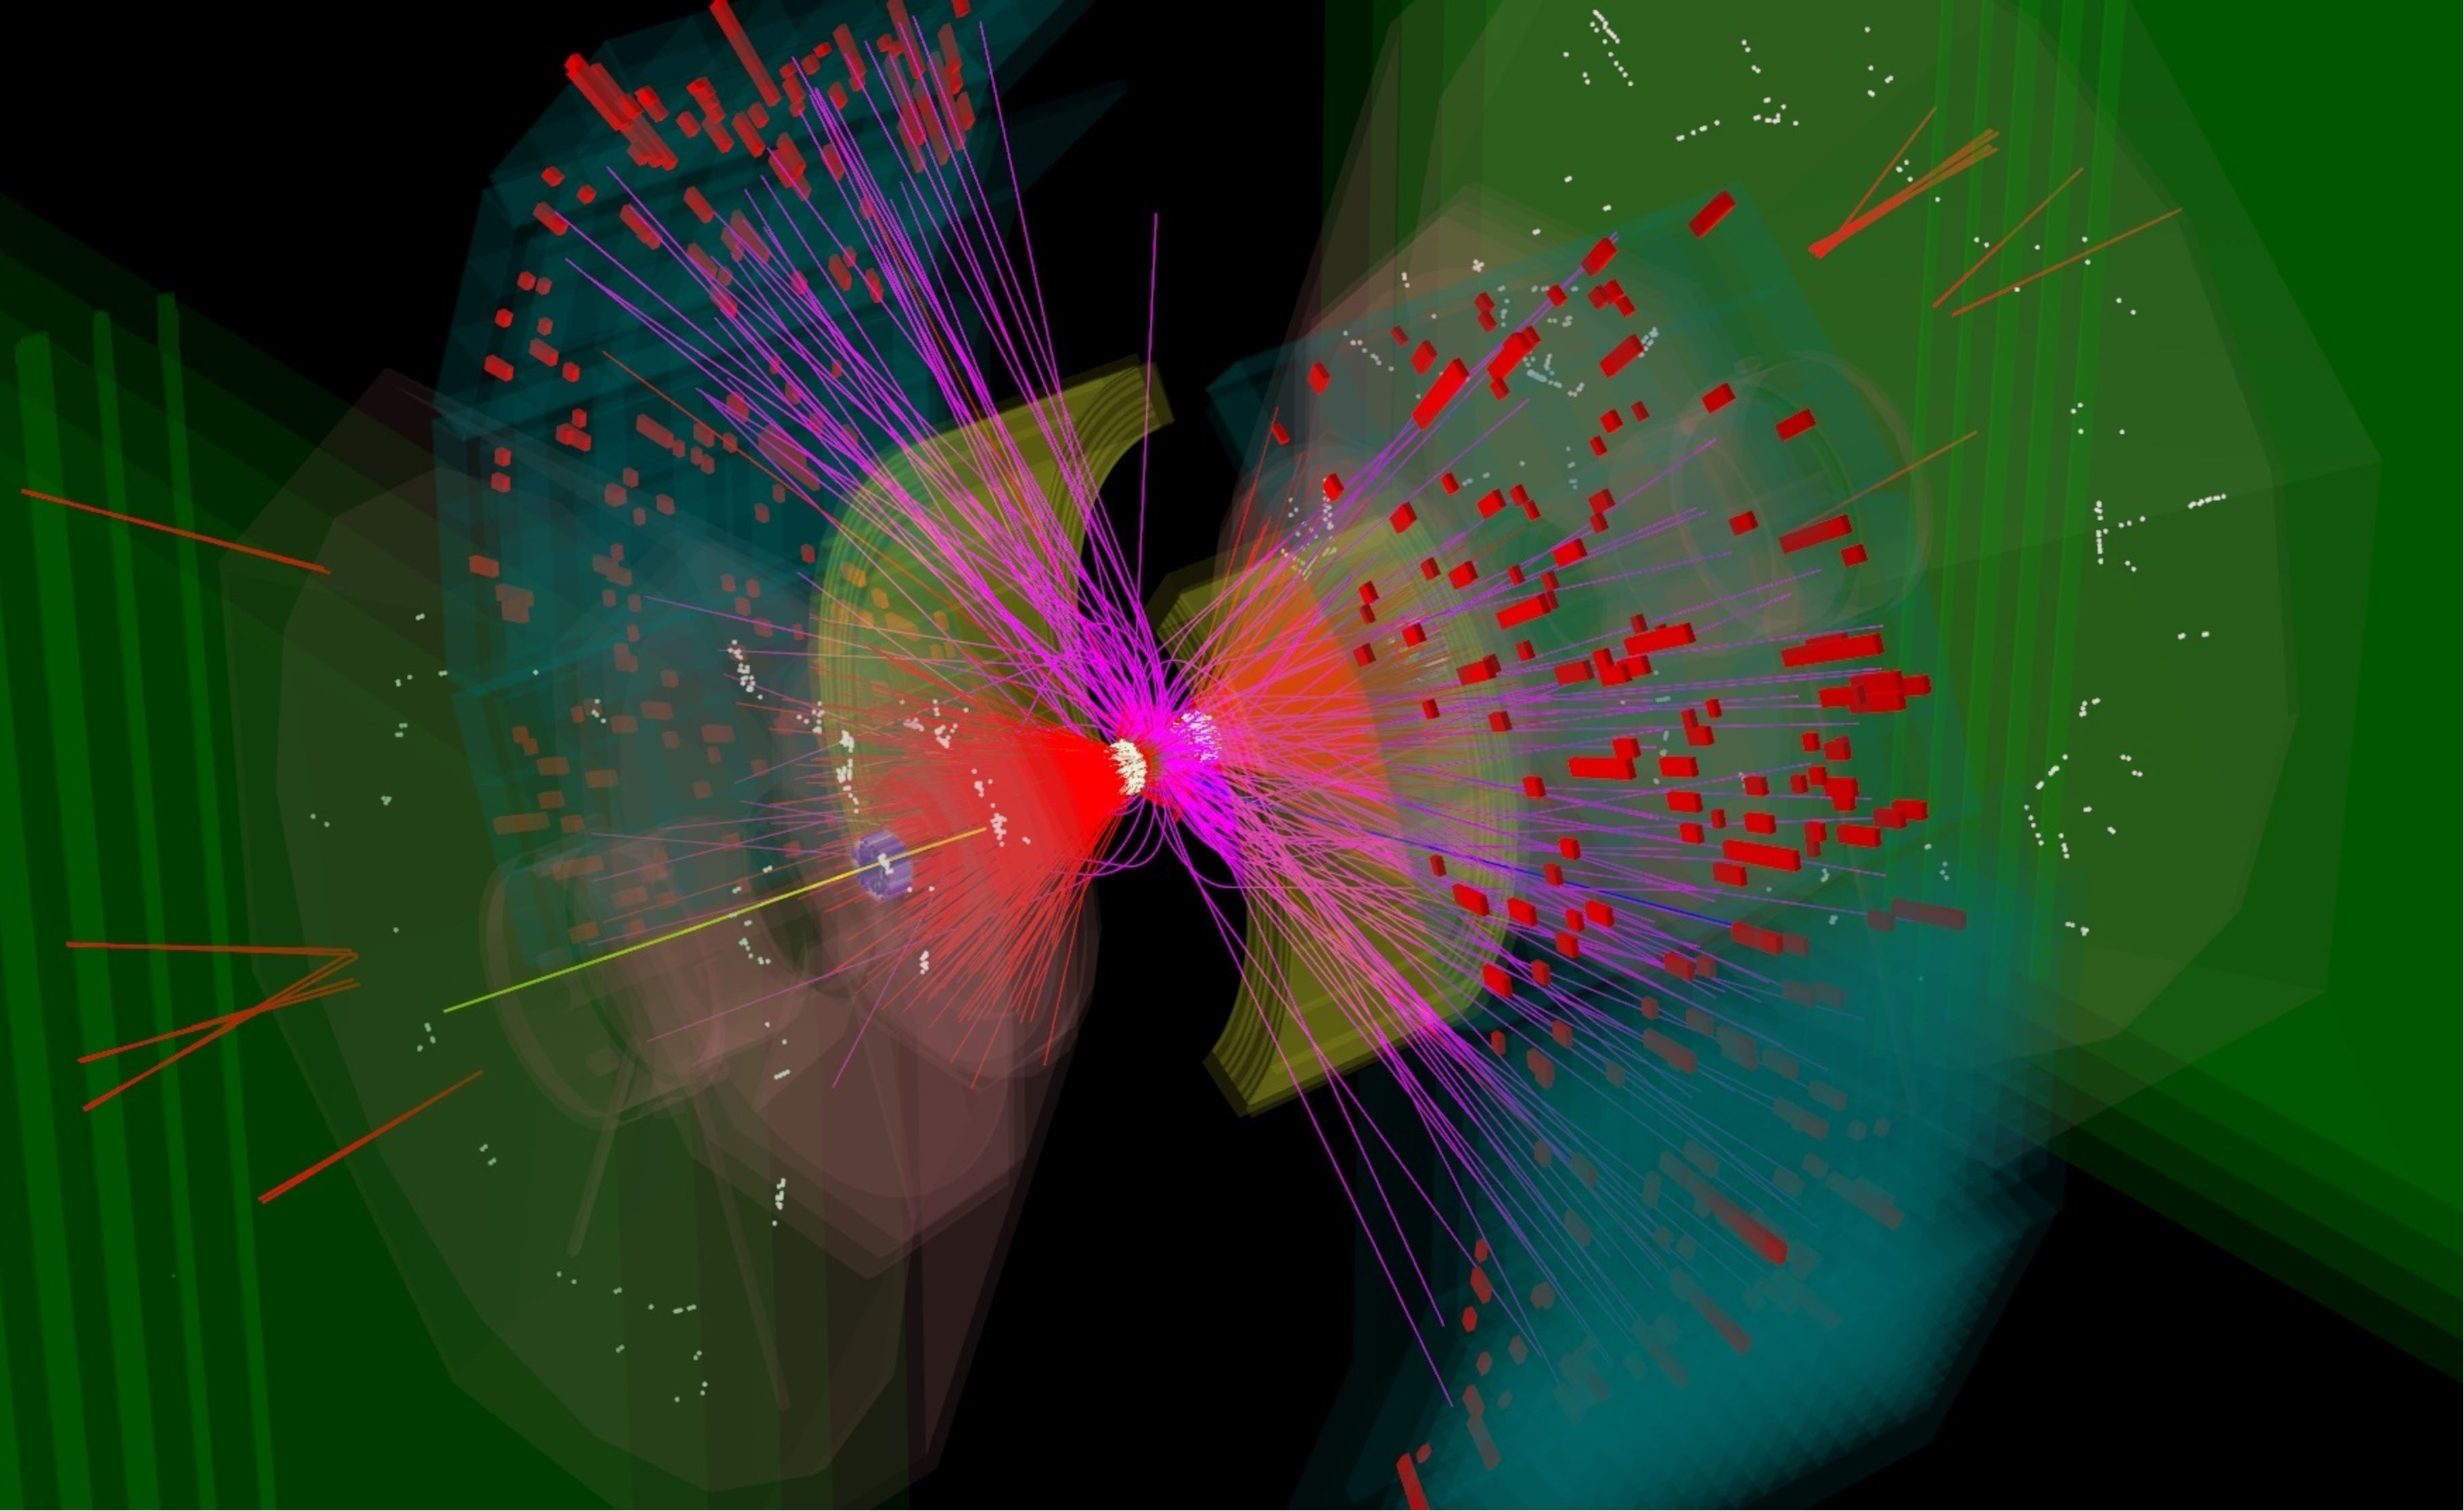
\includegraphics[width=0.7115\textwidth]{figs/collision.pdf}\\\vspace{2pt}
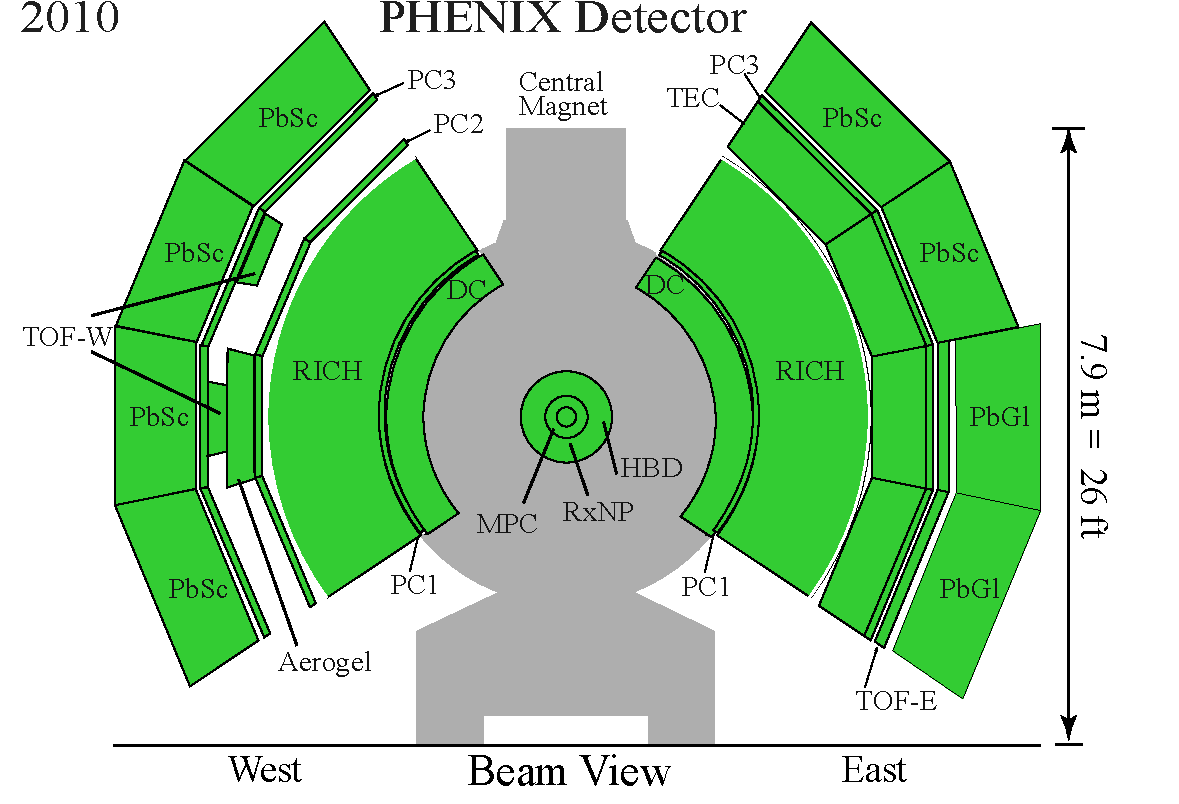
\includegraphics[width=0.8100\textwidth]{figs/Phenix_2010_v2.pdf}
\end{center}
\begin{tightitemize}\vspace{-0.022\textheight}
%\item Observing collisions of p,$\;$d,$\;$Cu,$\;$Au,$\;$Al,$\;$He,$\;$U
\item Charged pion ID from $\sim$ 0.2 to 2 GeV/c
\end{tightitemize}
\vspace{-11pt}
}

\headerbox{Introduction to three particle Bose-Einstein correlations}{name=fff,span=2,column=1,row=0,headerFontColor=black}{
\begin{tightitemize}
\item Invariant momentum distributions: $N_1(p_i), N_2(p_1,p_2),N_3(p_1, p_2, p_3)$
\item The definition of the correlation function:
\end{tightitemize}
\vspace{-0.015\textheight}
\begin{align*}
C_n(p_1,\dots,p_n)=\frac{N_n(p_1,\dots,p_n)}{N_1(p_1)\cdots N_1(p_n)}\textnormal{, for chaotic emission: }
N_n(x_1,\dots,x_n)=\int \prod_{i=1}^{n}S(x_i,p_i)|\Psi_{n}(\{x_i\})|^2 d^4x_1\dots d^4x_n
\end{align*}
\vspace{-0.015\textheight}
\begin{tightitemize}
  \setlength\itemsep{0.3em}
\item $S(x,p)$ source function (usually assumed to be Gaussian - Levy is more general)
\item $\Psi_n$ $n$-particle wave function - interaction free case: symmetrized combination of plane waves $\rightarrow C_n^{(0)}$
\item Coordinate transformation: $q_{ij}=p_i-p_j \Longrightarrow C_3(q_{12},q_{13},q_{23})$ for various $p_T=|p_{T1}+p_{T2}+p_{T3}|/3$
\item Longitudinal co-moving system of triplet: $k_{ij}=|q_{ij}^{\mathrm{LCMS3}}|$
\item Three dimensional correlation function: $C_3(k_{12}, k_{13}, k_{23})$
\end{tightitemize}
\vspace{-0.008\textheight}

%\begin{tightitemize}
%\item Sometimes this simple formula fails (cf. experimentally observed oscillations at L3, CMS)
%\end{tightitemize}
}

\headerbox{Final state interactions, pion production mechanisms}{name=ff1,column=1,row=1,below=fff,span=2,headerFontColor=black}{
\begin{tightitemize}
\item Identical charged pions - Coulomb interaction distort the simple picture
\item Coulomb-corrected correlation: $C_{3}(k_{12}, k_{13}, k_{23}) = K_3(k_{12}, k_{13}, k_{23})\cdot C_{3}^{(0)}(k_{12}, k_{13}, k_{23})$
\item Coulomb-correction from Generalized Riverside \cite{gr1,gr2}: $K_3(k_{12}, k_{13}, k_{23})\approx K_1(k_{12})K_1(k_{13})K_1(k_{23})$
\item Resonance pions contribute to the full source: $S=S_{\rm core}+S_{\rm halo}$
\item Reduce the measurable correlation function to $C_2(0)=1+\lambda_2$ with $\lambda_2=f_c^2=\left(\frac{\rm core}{\rm core+halo}\right)^2$\cite{corehalo1, corehalo2}
\item Non-chaotic emission also possible; coherent fraction: $p_c=\frac{\rm coherent}{\rm coherent+incoherent}$
\end{tightitemize}
}
\vspace{-0.1\textheight}

\headerbox{The Levy-distribution and the three particle correlation strength}{name=ff2,column=0,row=2,below=aaa,span=2,headerColorOne=darkorange1,headerColorTwo=darkorange2}{
\begin{tightitemize}
\item Generalized Gaussian from anomalous diffusion: Levy-distribution, $\alpha=2$: Gauss, $\alpha=1$: Cauchy\vspace{-0.005\textheight}
\vspace{-4pt}
\begin{align*}
\mathcal{L}(\alpha,R,r)=(2\pi)^{-3} \int d^3q e^{iqr} e^{-\frac{1}{2}|qR|^{\alpha}}
\end{align*}
\vspace{-16pt}
\item Interaction free correlation function with Levy source:
\vspace{-9pt}
\begin{align*}
C_3^{(0)}(k_{12}, k_{13}, k_{23}) = 1+ \ell_3e^{-0.5\big(|2k_{12}R|^\alpha+|2k_{13}R|^\alpha+|2k_{23}R|^\alpha\big)}
+\ell_2\Big(e^{|2k_{12}R|^\alpha}+e^{|2k_{13}R|^\alpha}+e^{|2k_{23}R|^\alpha}\Big)
\end{align*}
\vspace{-15pt}
\item Three particle correlation strength: $\lambda_3 \equiv C_3(k_{12}=k_{13}=k_{23}=0)-1=\ell_3+3\ell_2$
\vspace{3pt}
\item Core-Halo independent parameter: $\kappa_3=\big(\lambda_3-3\lambda_2\big)/\big(2\lambda_2^{3/2}\big)$, where $\lambda_2\equiv C_2(k=0)-1$ (two particle corr. strength) \vspace{-10pt}
\end{tightitemize}
}

%\headerbox{Example diagonal correlation function}{name=ccc,column=2,below=ff1,row=2,headerColorOne=darkorange1,headerColorTwo=darkorange2}{
%\begin{center}
%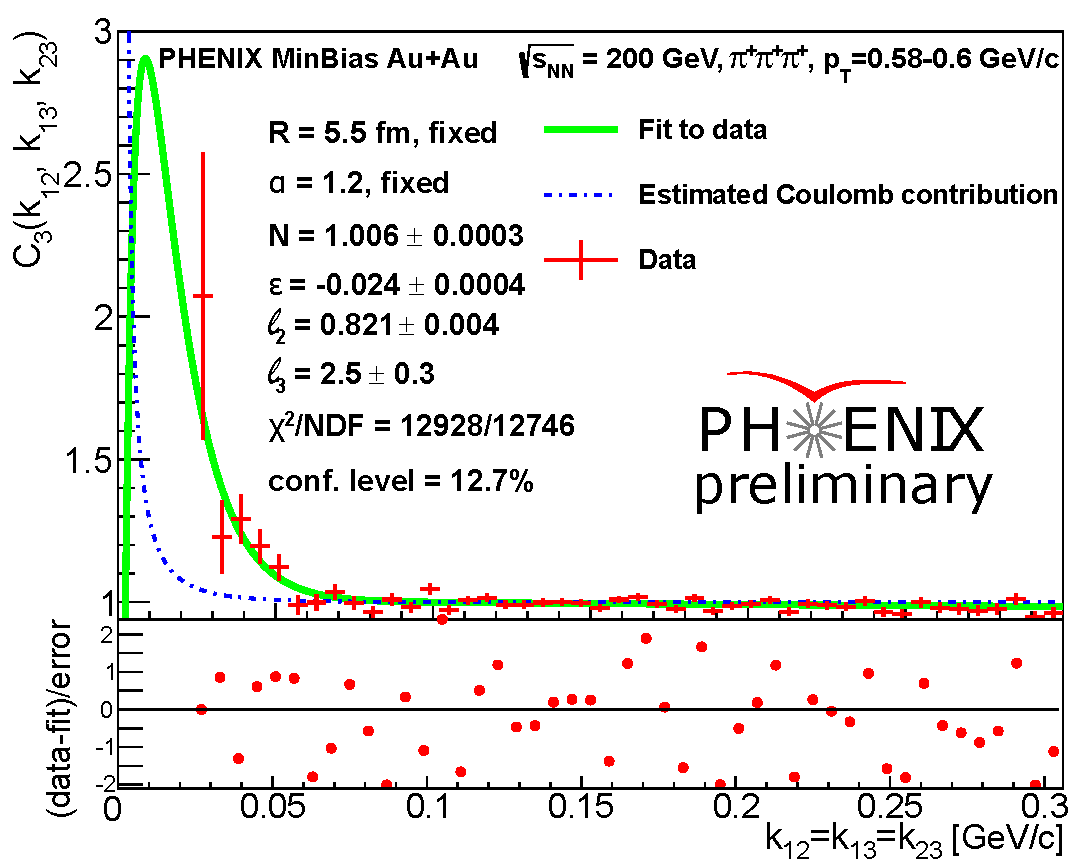
\includegraphics[width=1\textwidth]{res/diag_highpt}
%\end{center}
%}

\headerbox{{\fontsize{11.25}{0}\selectfont Partial coherence ($p_c$) vs fractional core ($f_c$)}}{name=ccc,column=2,below=ff1,row=2,headerColorOne=darkorange1,headerColorTwo=darkorange2}{
\begin{tightitemize}
\item Simple theoretical model \cite{fcpc}: $\lambda_2(f_c, p_c)$, $\lambda_3(f_c, p_c)$ 
\item Measured $\lambda_2^{\rm meas.} \rightarrow\\ \lambda_2^{\rm meas.}=\lambda_2(f_c,p_c) \Longrightarrow f_c(p_c)$ (green lines)
\item Measured $\lambda_3^{\rm meas.} \rightarrow\\ \lambda_3^{\rm meas.}=\lambda_3(f_c,p_c) \Longrightarrow f_c(p_c)$ (blue lines)
\item Example 2D plot at $m_T=0.36$ GeV$/c^2$:
\end{tightitemize}
\begin{center}
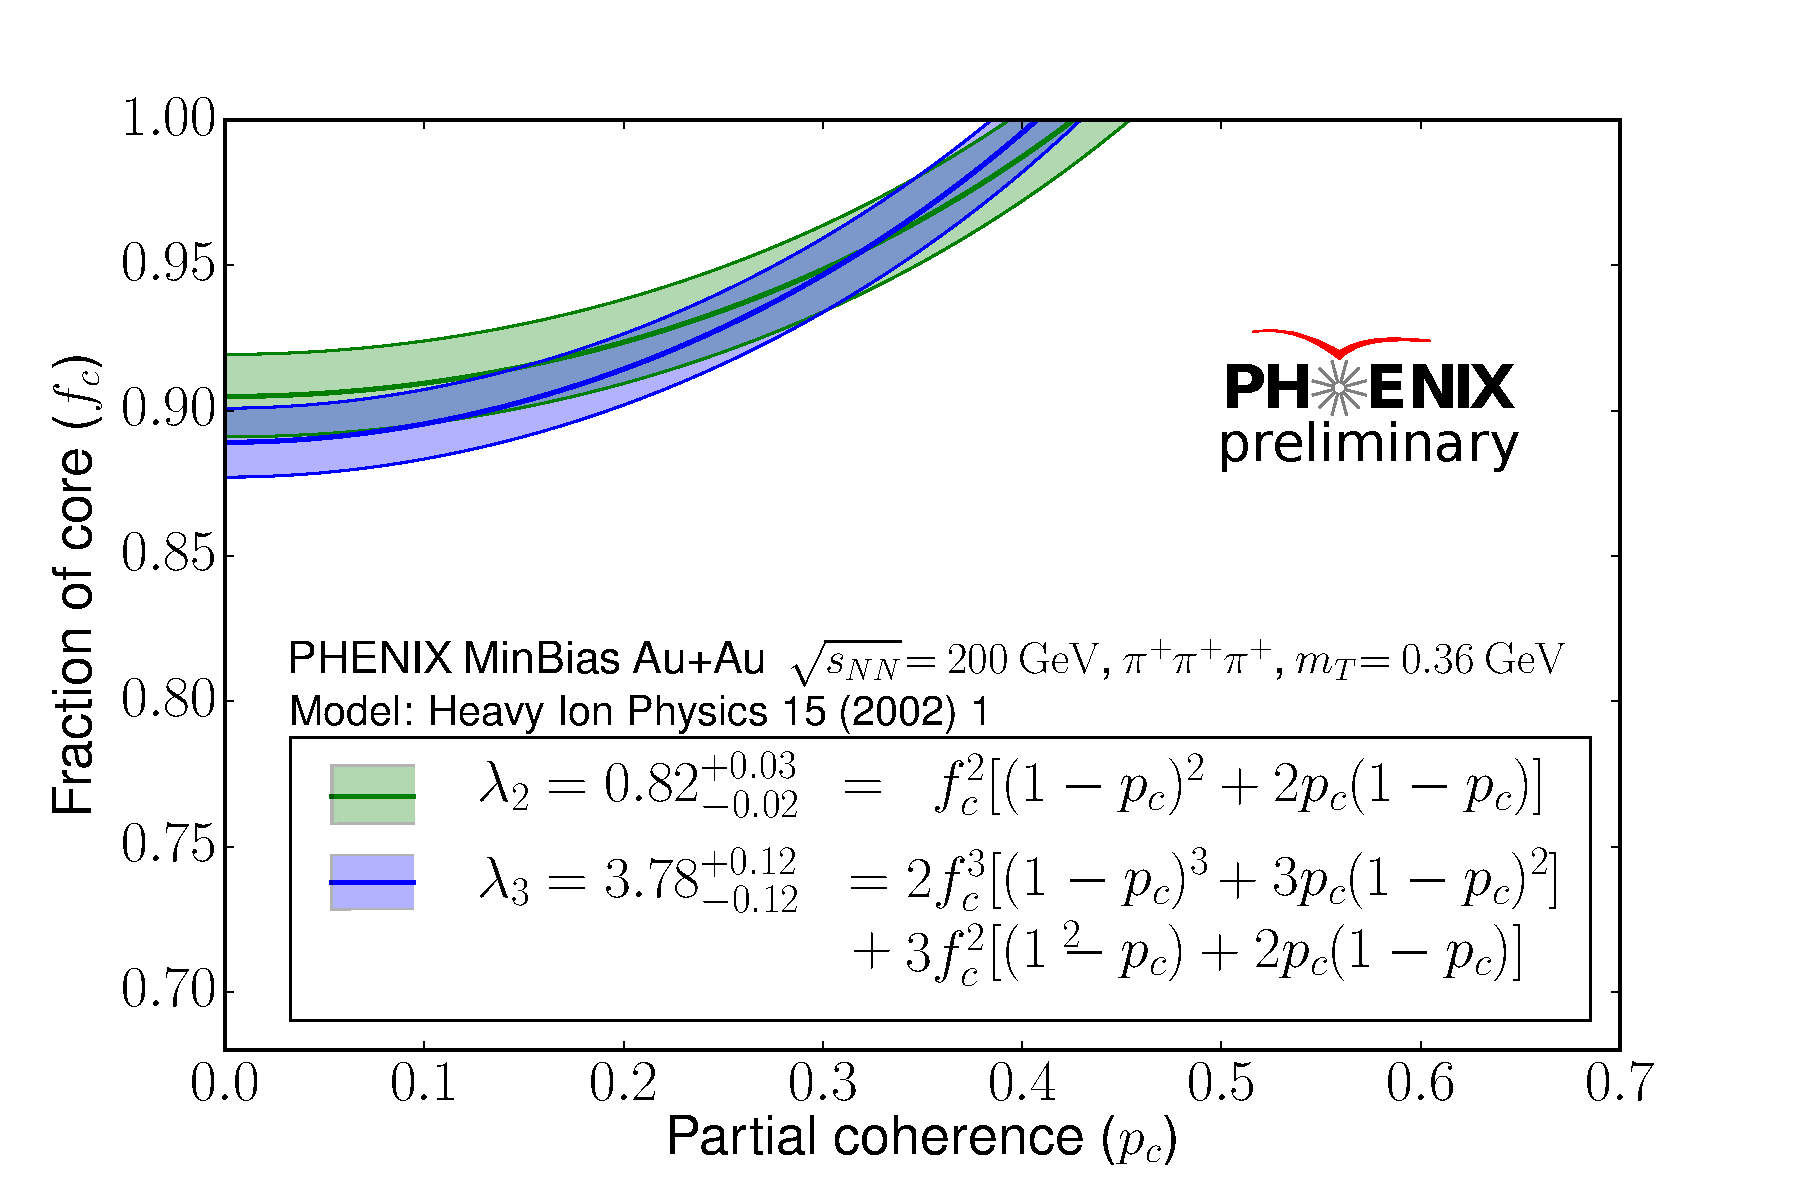
\includegraphics[width=1.0\textwidth]{res/cropped_fcpc2}
%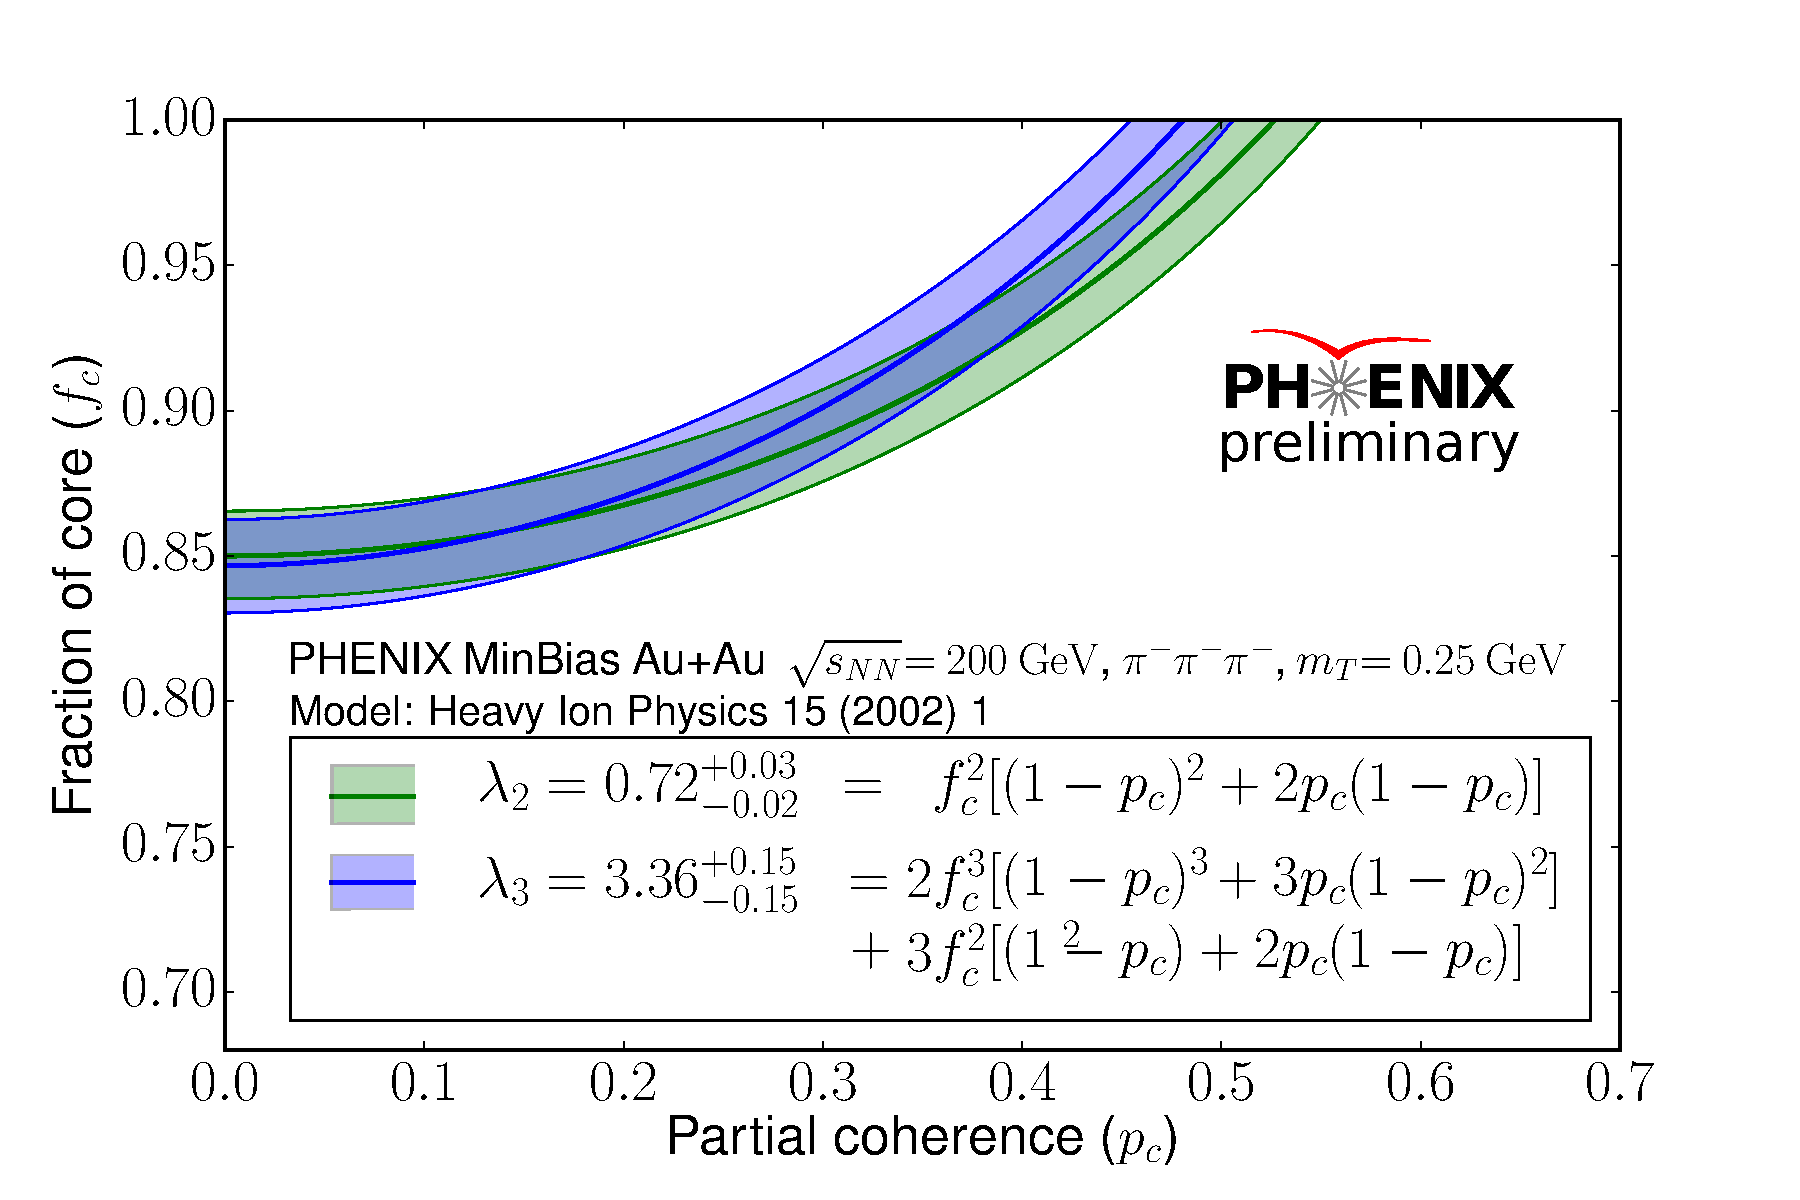
\includegraphics[width=0.49\textwidth]{res/cropped_fcpc1}
\end{center}
}

\headerbox{Correlation strength $\lambda_3$ is within core-halo + chaotic emission range of $[0,5]$ for all $m_T$}{name=gg1,column=0,span=2,below=ff2,row=3,headerColorOne=darkpurple1,headerColorTwo=darkpurple1}{
\begin{center}
\hspace*{-0.20cm}
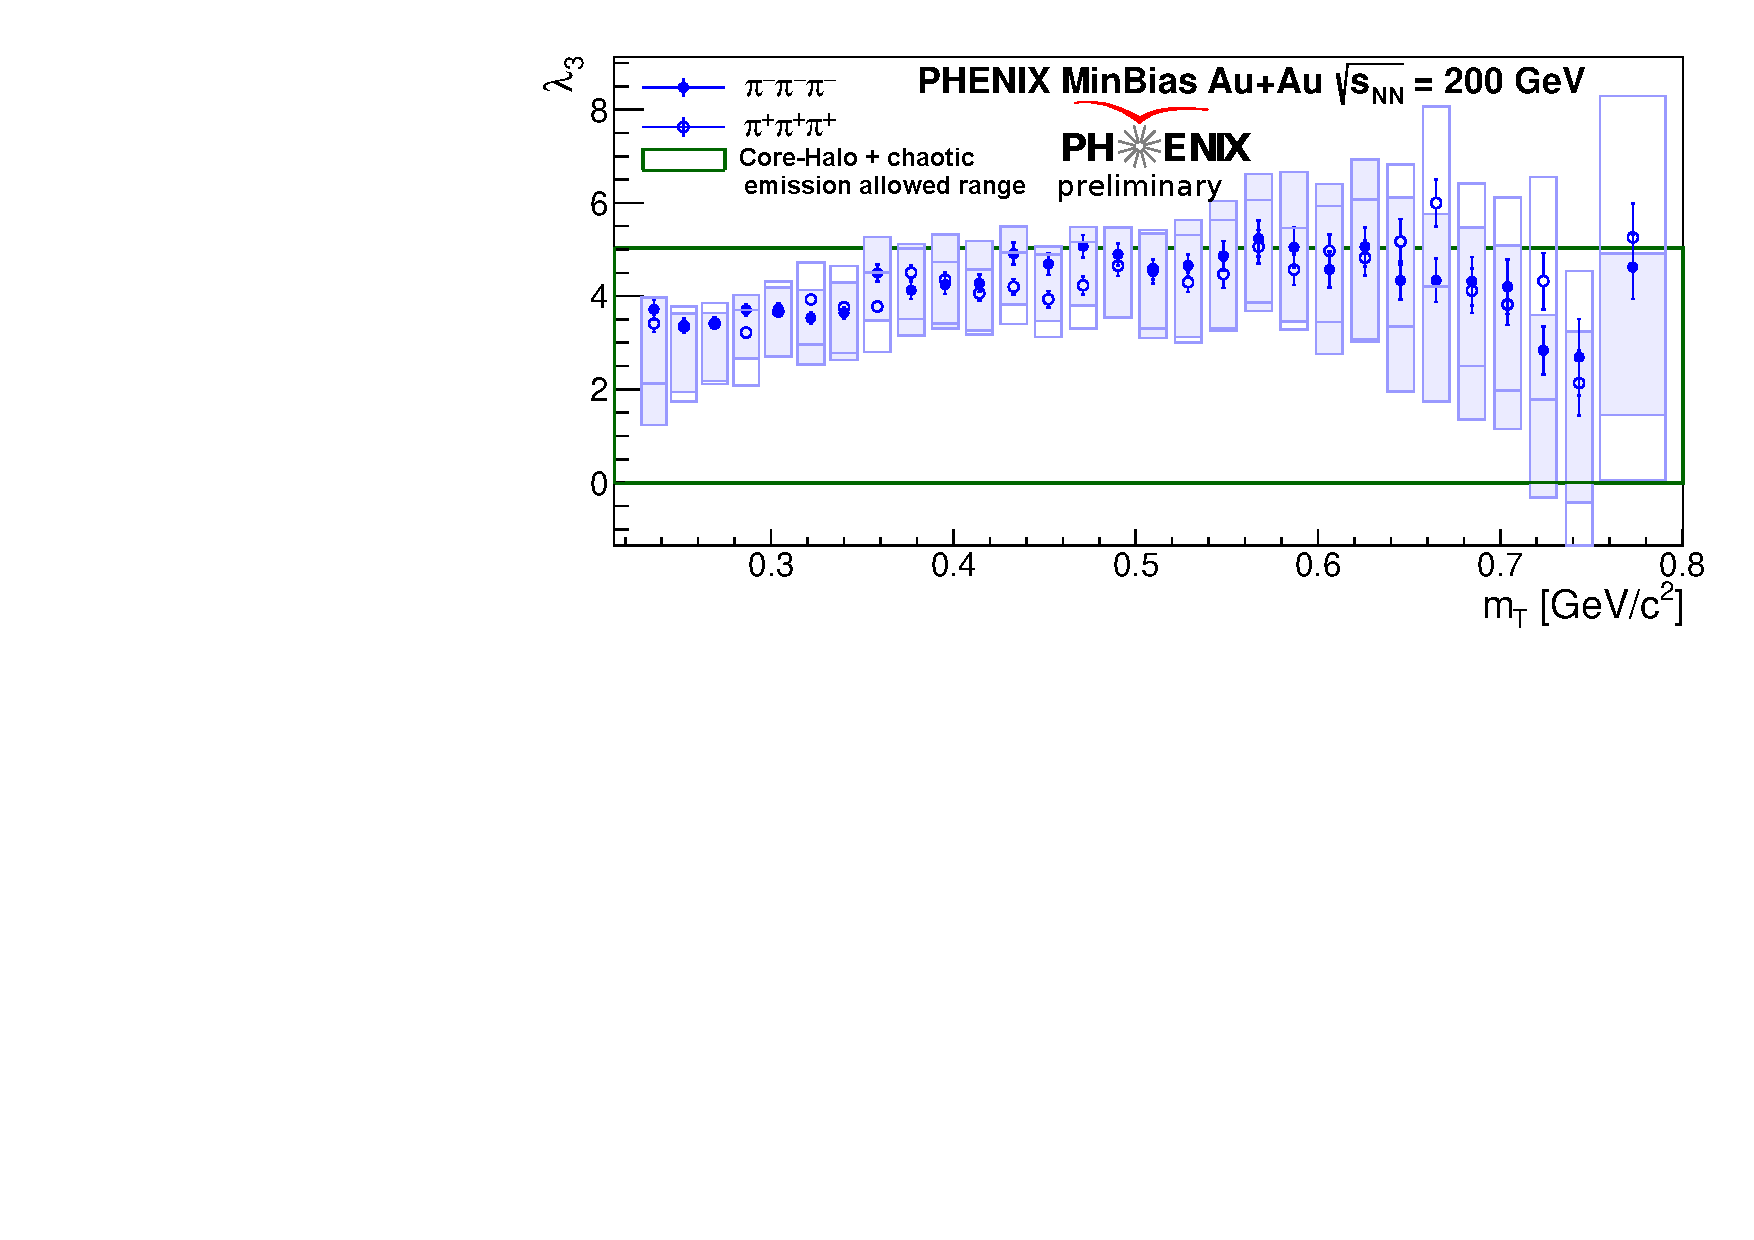
\includegraphics[width=0.85\textwidth]{res/lambda3}
\vspace*{-0.25cm}
\end{center}
}

\headerbox{Core-halo independent parameter $\kappa_3$ vs $m_T$: $\kappa_3\neq1$ is statistically significant} {name=sum,column=0,above=bottom,row=4,span=2,headerColorOne=darkpurple1,headerColorTwo=darkpurple2}{
\begin{center}
\hspace*{-0.20cm}
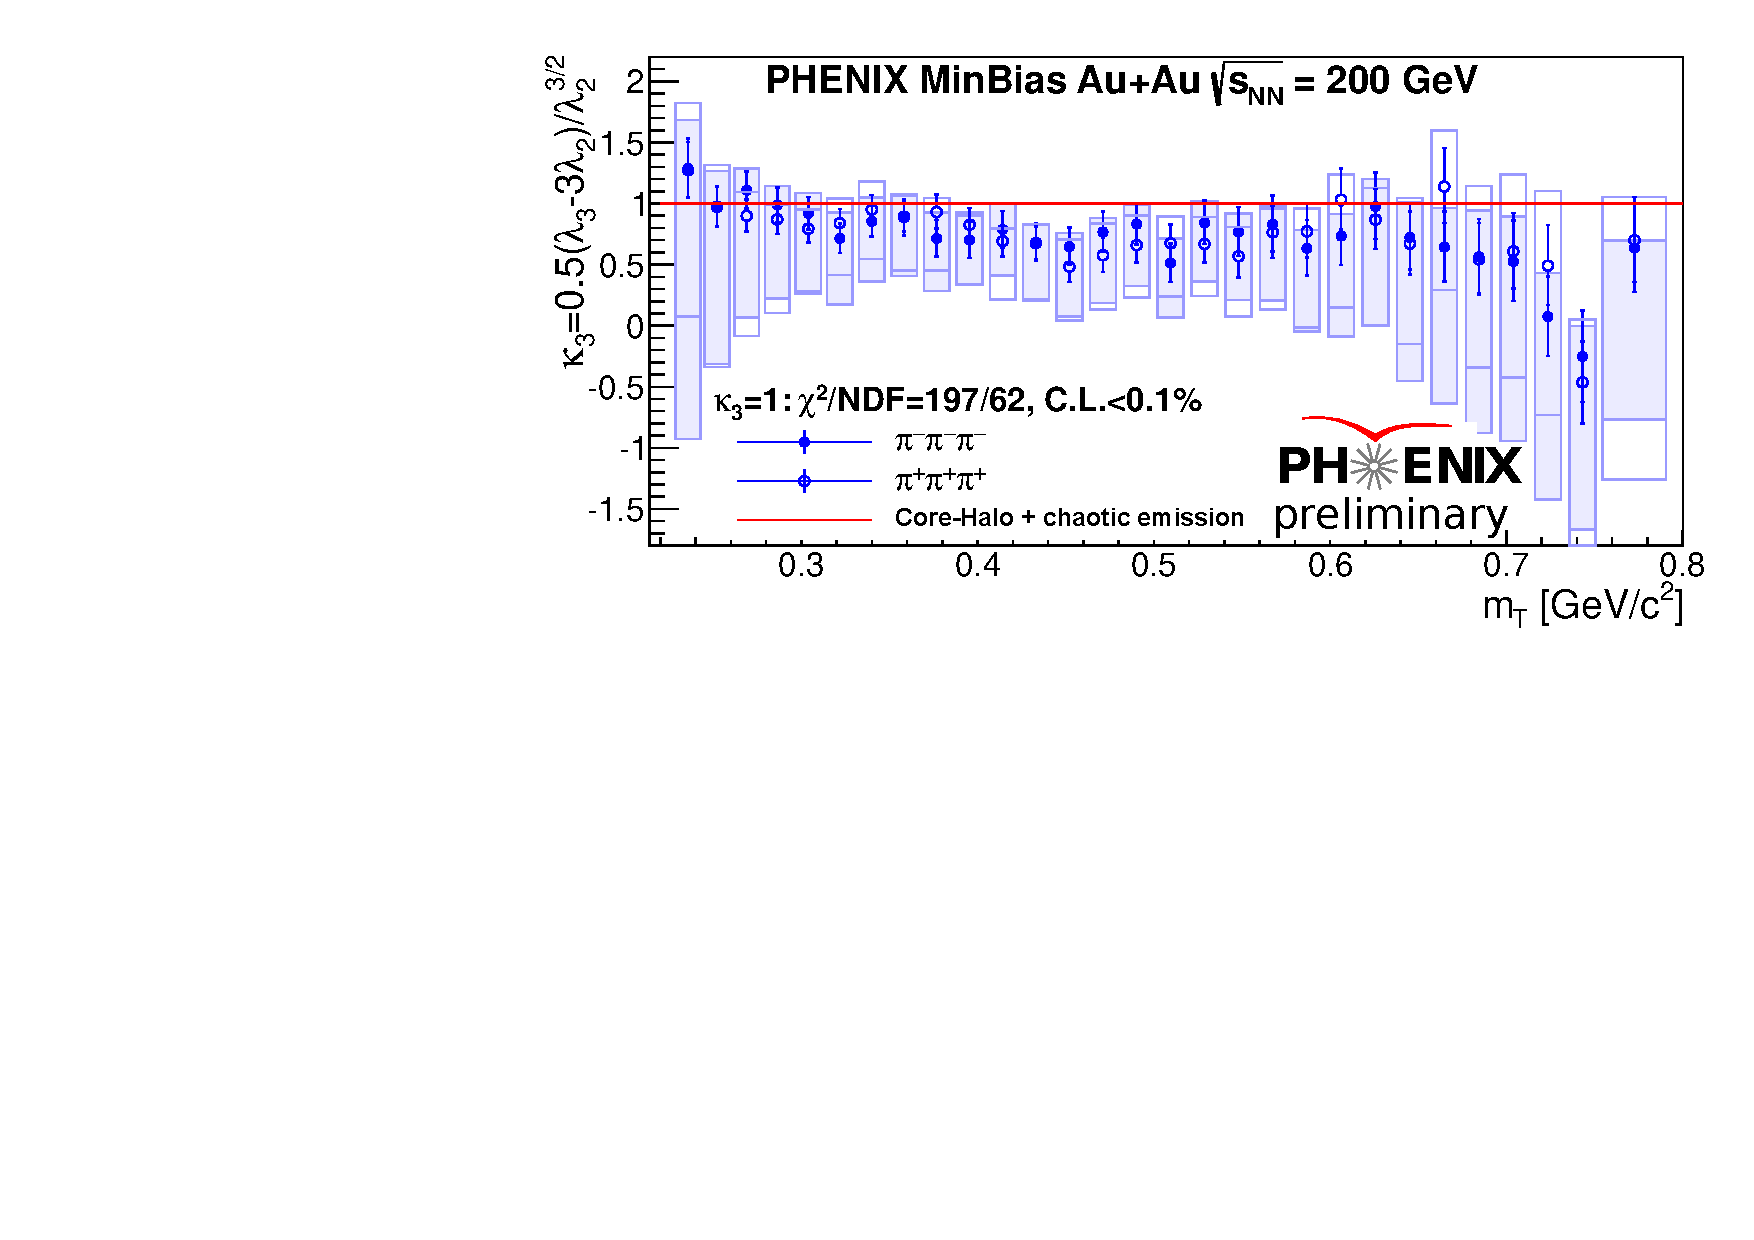
\includegraphics[width=0.85\textwidth]{res/kappa3}
\vspace*{-0.25cm}
\end{center}
}

%\headerbox{Core-Halo independent parameter $\kappa_3$ vs. $m_T$}{name=gg2,column=1,below=ff2,headerColorOne=darkpurple1,headerColorTwo=darkpurple2}{
%\begin{tightitemize}
%\item Empirically found, linear in $m_T$
%\item Physical interpretation still an open question
%\end{tightitemize}
%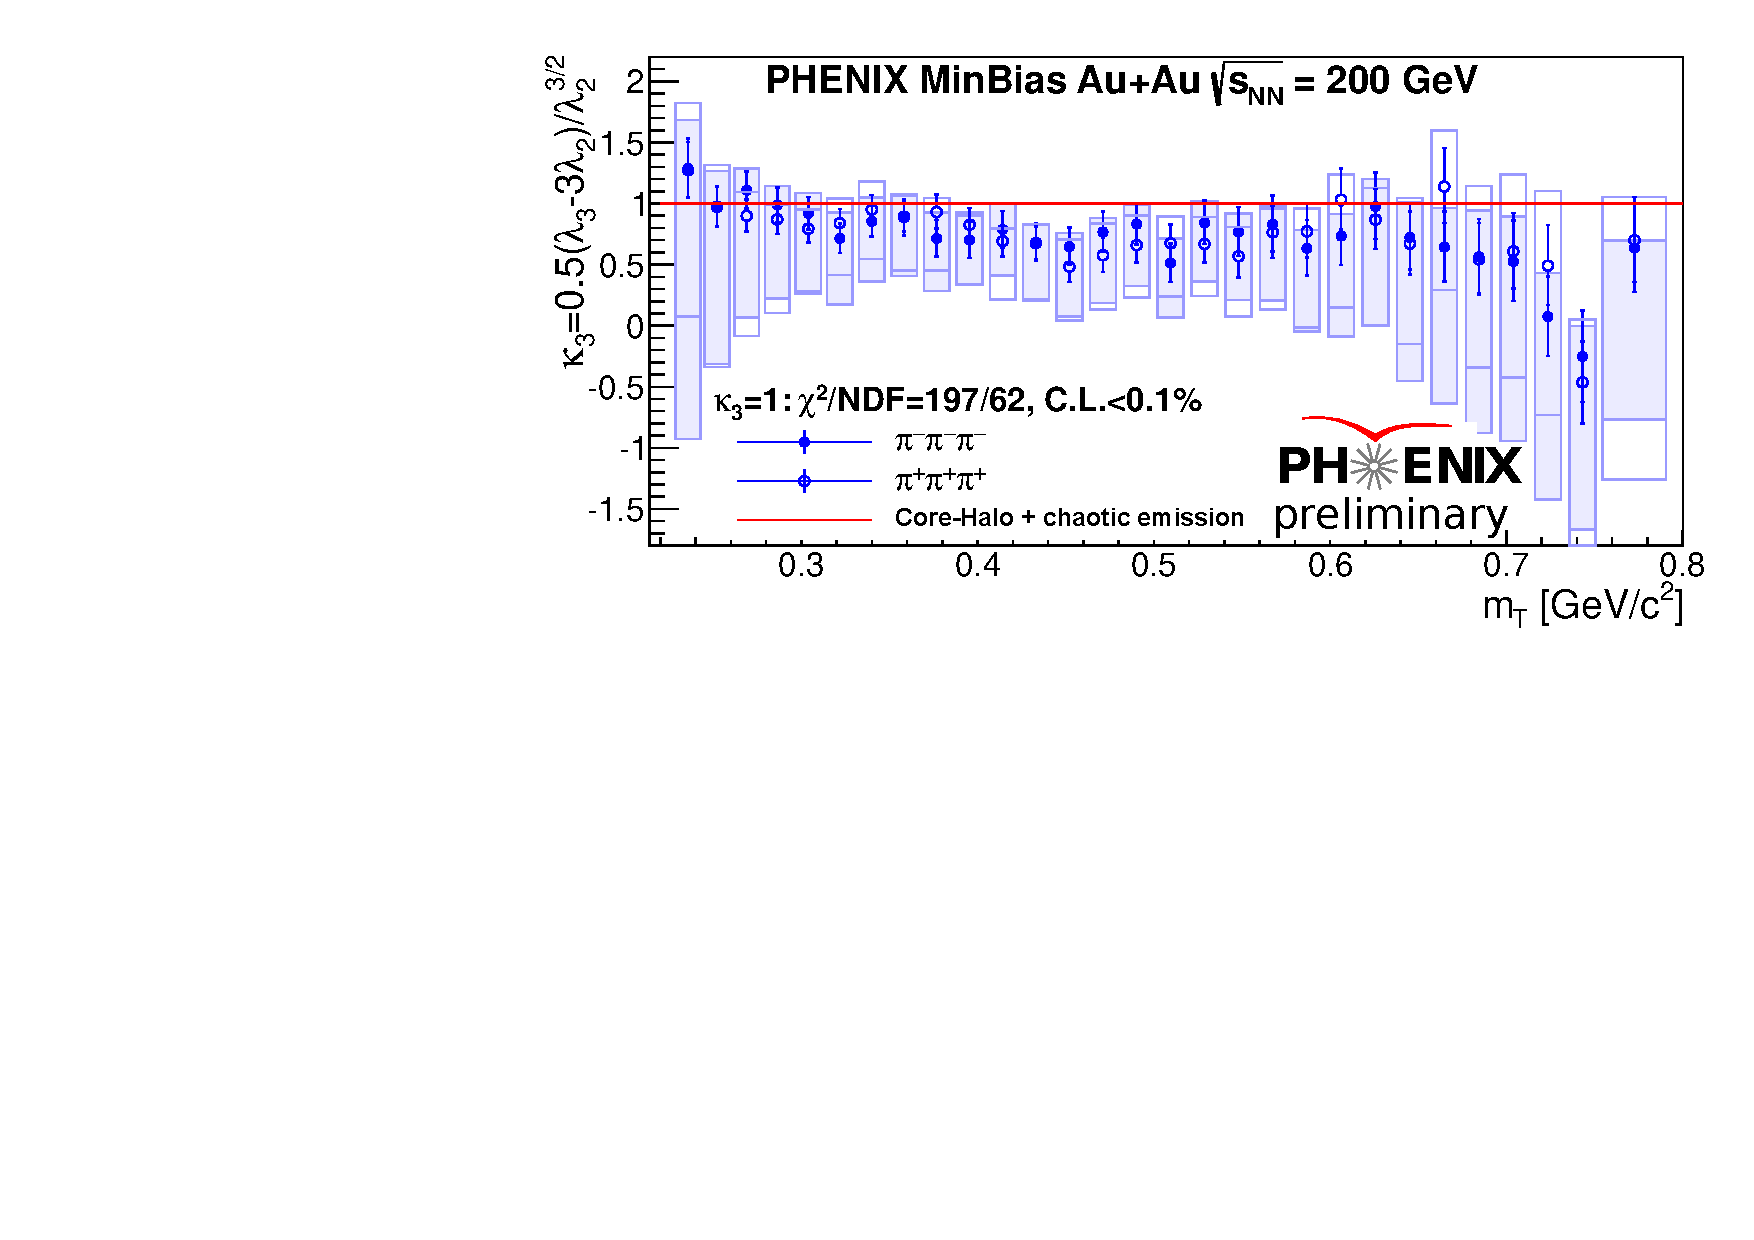
\includegraphics[width=1.014\textwidth]{res/kappa3}
%}

%\headerbox{Partial coherence}{name=sum,column=0,above=bottom,row=4,span=2,headerColorOne=darkpurple1,headerColorTwo=darkpurple2}{
%\begin{tightitemize}
%\item Fraction of core: $f_c=\frac{\rm core}{\rm core+halo}$, fraction of coherently produced pions:  $p_c=\frac{\rm coherent}{\rm coherent+incoherent}$
%\item Simple theoretical model \cite{fcpc}: $\lambda_2(f_c, p_c)$, $\lambda_3(f_c, p_c)$ 
%\item Measured $\lambda_2^{\rm meas.}$ $\rightarrow$ $\lambda_2^{\rm meas.}=\lambda_2(f_c,p_c)$ $\Longrightarrow$ $f_c(p_c)$ (green lines)
%\item Measured $\lambda_3^{\rm meas.}$ $\rightarrow$ $\lambda_3^{\rm meas.}=\lambda_3(f_c,p_c)$ $\Longrightarrow$ $f_c(p_c)$ (blue lines)
%\end{tightitemize}
%\begin{center}
%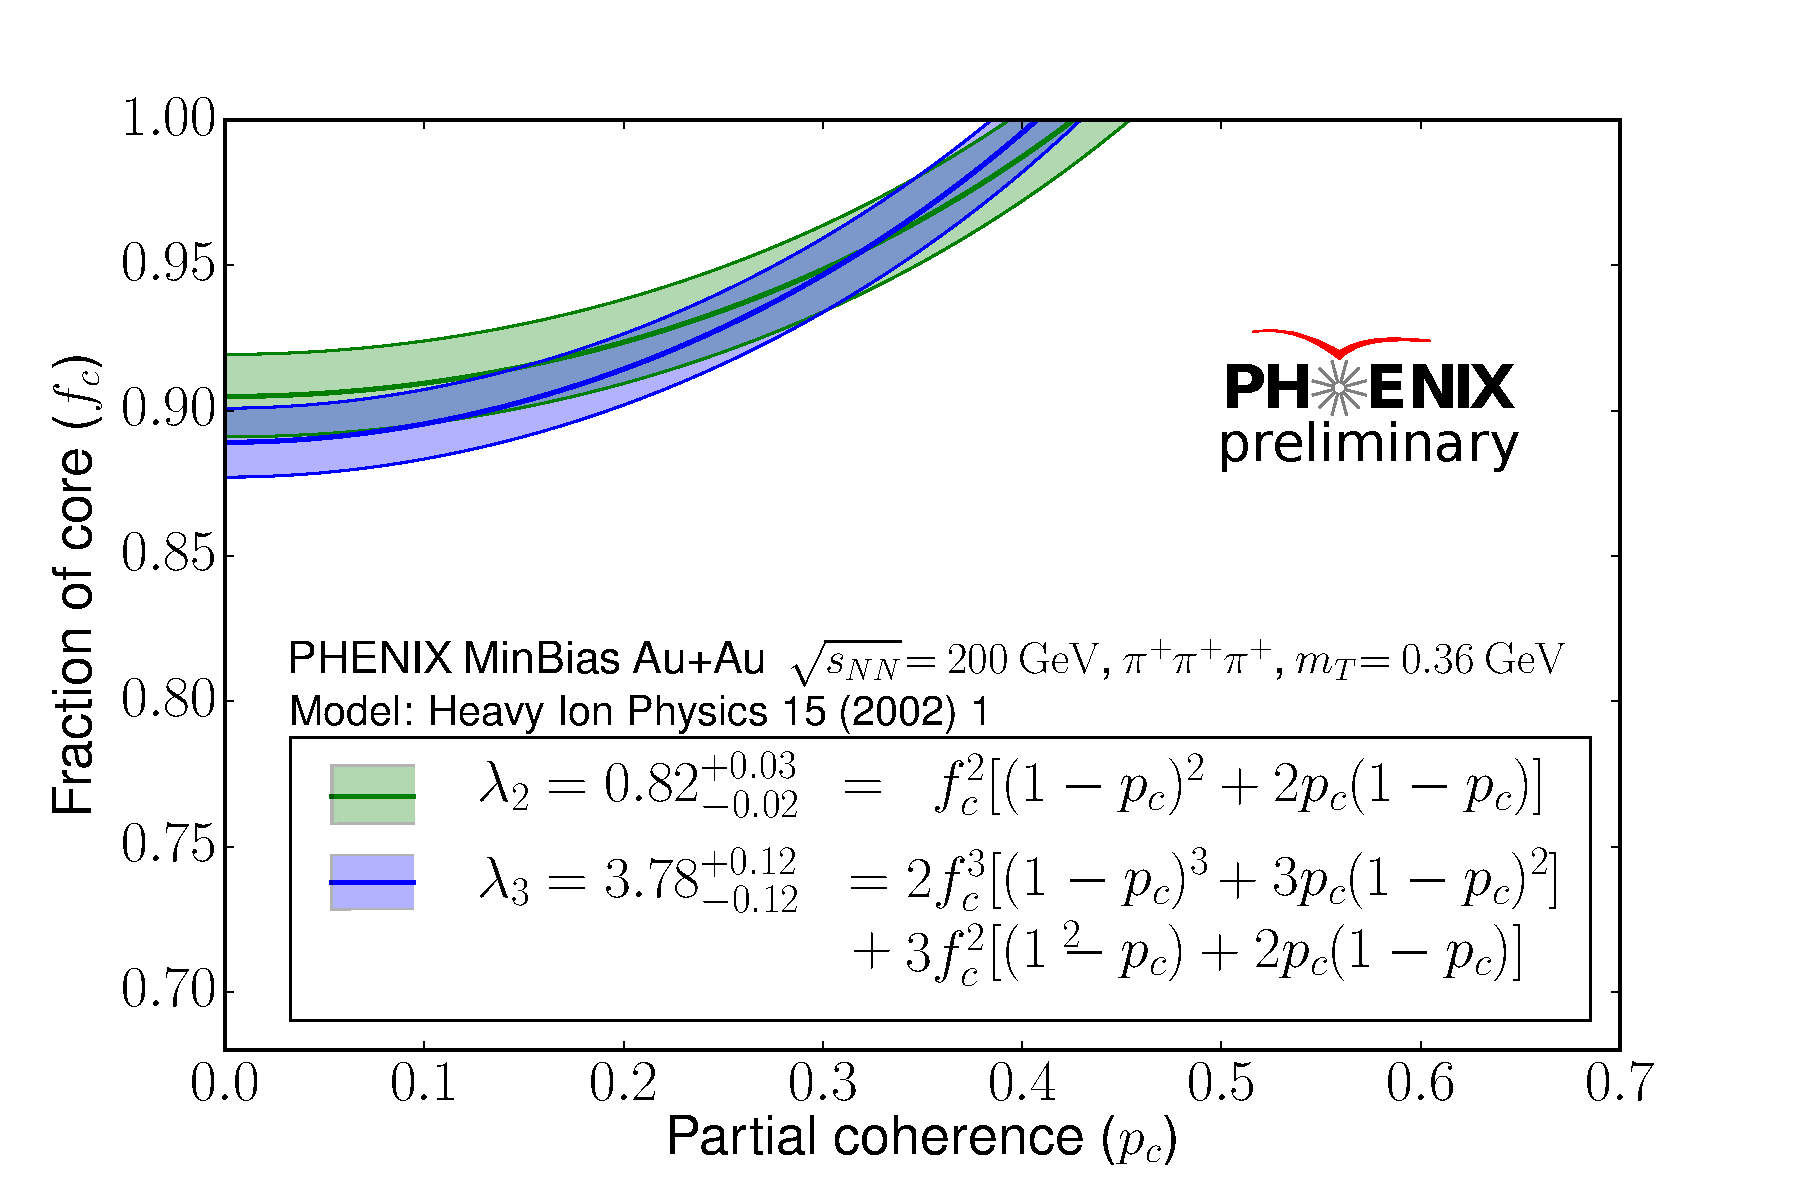
\includegraphics[width=0.49\textwidth]{res/cropped_fcpc2}
%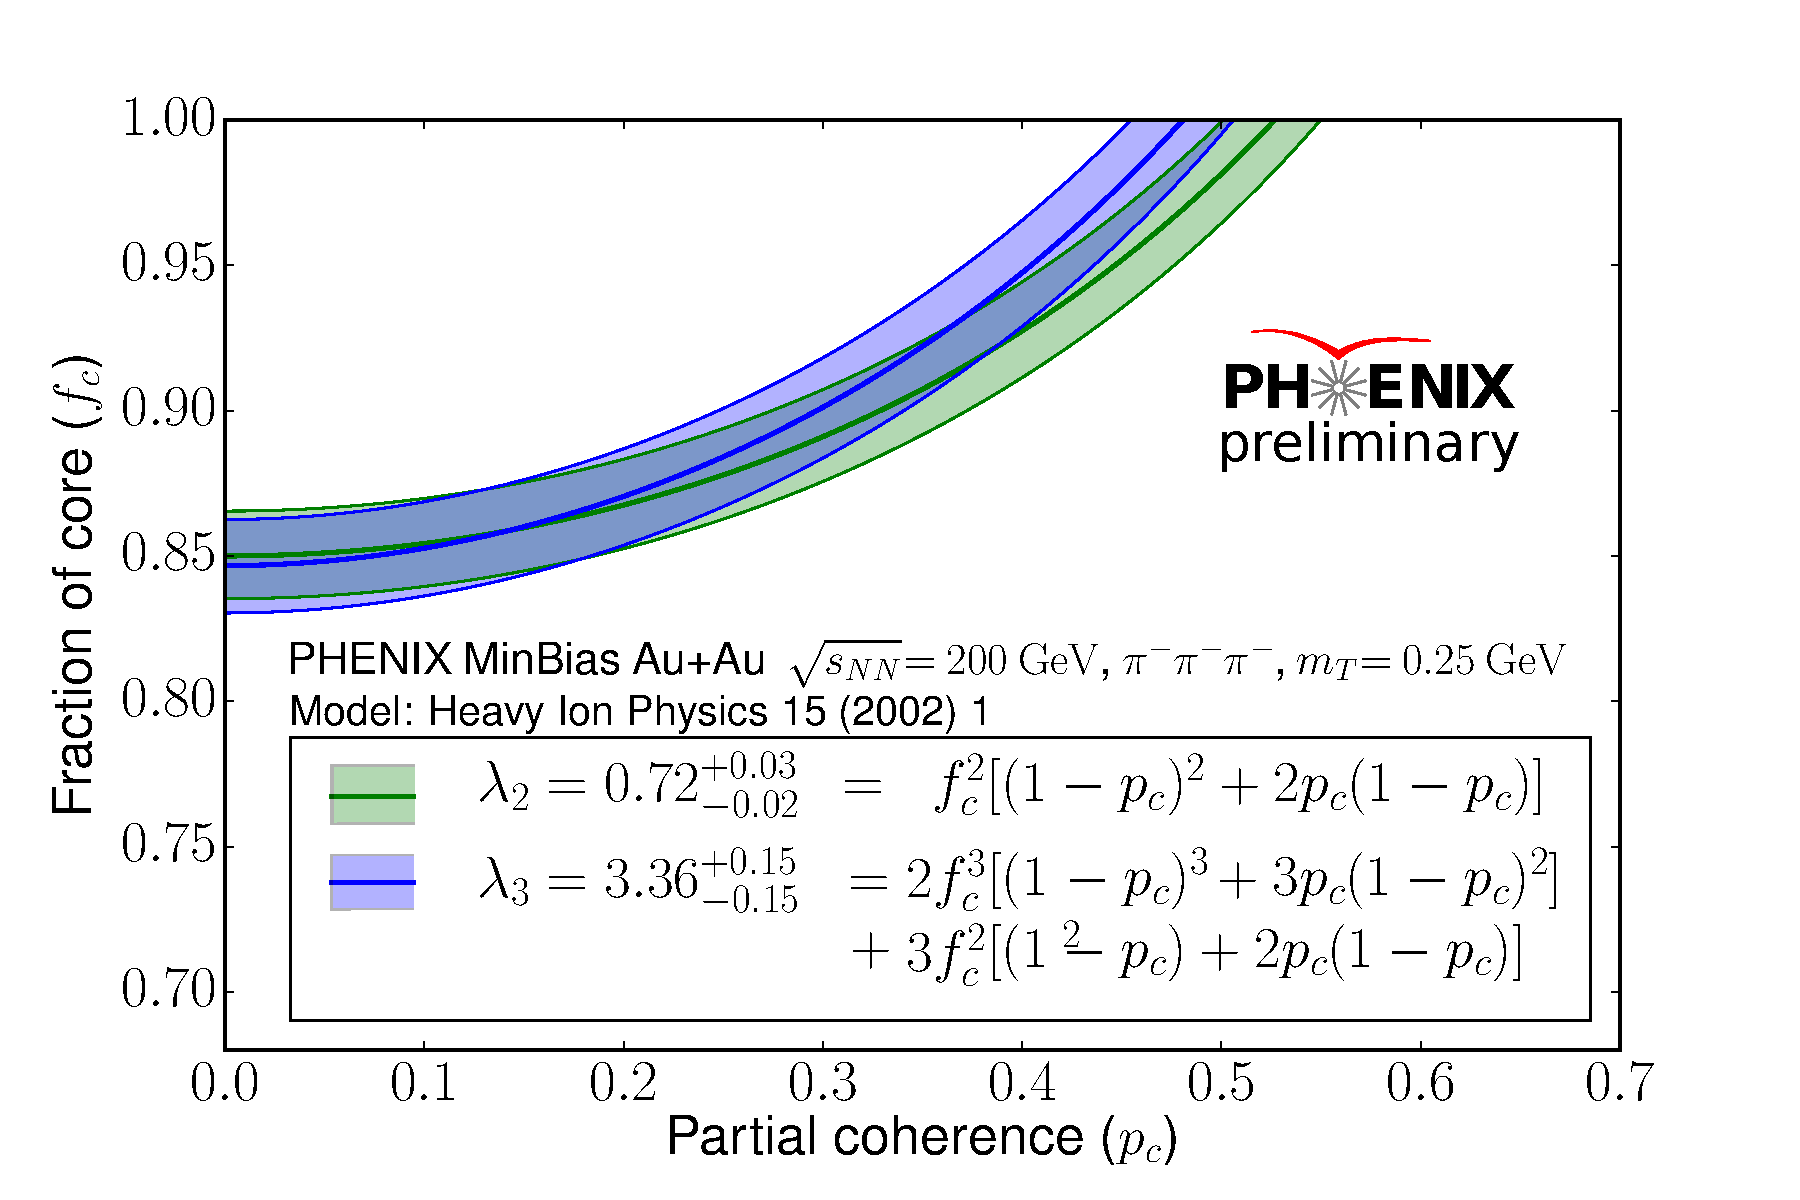
\includegraphics[width=0.49\textwidth]{res/cropped_fcpc1}
%\end{center}
%}

%\headerbox{Newly found scale param. $\widehat{R}$ vs. $m_T$}{name=rht,column=1,row=4,above=bottom,headerColorOne=darkpurple1,headerColorTwo=darkpurple2}{
%\begin{center}
%\includegraphics[width=1.\textwidth]{chopped_results/rhat_preliminary_stamp}
%\end{center}
%\begin{tightitemize}\vspace{-0.023\textheight}
%\item Empirically found, linear in $m_T$
%\item Physical interpretation still an open question
%\end{tightitemize}
%}

\headerbox{Summary}{name=ddd,column=2,below=ccc,headerColorOne=darkpurple1,headerColorTwo=darkpurple2}{
\begin{tightitemize}\addtolength{\itemsep}{-0.001\textheight}
\item 3 pion B-E correlations with Levy-source are shown
\item Good agreement with data
\item $\lambda_3$ within Core-Halo + chaotic emission limits (0-5)
\item $\lambda_2$, $\lambda_3$ are consistent within $1\sigma$ region on $(f_c, p_c)$ plots
\item Core-Halo + chaotic emission $\kappa_3=1$
\item Statistically significant deviation from $\kappa_3=1$
\item Statistically significant exclusion region:\\ analyzed at $m_T=0.36$ GeV$/c^2$\vspace{-0.004\textheight}
\begin{tightitemize}\addtolength{\itemsep}{-0.001\textheight}
\item $f_c<0.82$ can be excluded
\item $p_c>0.5$ can be excluded
\item Small ($p_c < 0.5$) partial coherence \\cannot be excluded\vspace{-0.002\textheight} \end{tightitemize}
\item Further $m_T$ regions will be investigated
\item $m_T$ dependent exclusion limits on $f_c,p_c$\\to be analyzed\vspace{-0.002\textheight}
\end{tightitemize}
}

\headerbox{References}{name=eee,column=2,below=ddd,above=bottom,headerColorOne=darkpurple1,headerColorTwo=darkpurple2}{
\renewcommand\refname{\vskip 0cm}
\begin{thebibliography}{9}\addtolength{\itemsep}{-0.006\textheight}
\small \vspace{-0.016\textheight}
\bibitem{gr1}{M. M. Aggarwal et al. (WA98 Collaboration) Phys. Rev. Lett. 85 2895 (2000)}
\bibitem{gr2}{J. Adams et al. (STAR Collaboration) Phys. Rev. Lett. 91 262301 (2003)}
\bibitem{corehalo1}{J. Bolz et al., Phys.Rev. D47 (1993) 3860}
\bibitem{corehalo2}{T. Cs�rg\H{o} et al., Z.Phys. C71 (1996) 491}
\bibitem{fcpc}{T. Cs�rg\H{o}, Heavy Ion Physics 15 (2002) 1}
\end{thebibliography}\vspace{-0.0075\textheight}
\scriptsize
{A.B. was 
\includegraphics[scale=0.03]{figs/emmi_logo_h1} supported by the �NKP-16-2 New National Excellence program of the Ministry of Human Capacities}
}

%\placetextbox{0.337}{0.8200}{\scalebox{1.}{\boldmath$\blacktriangleright$}}
%\placetextbox{0.666}{0.7425}{\scalebox{1.1}{\boldmath$\blacktriangledown$}}
%\placetextbox{0.500}{0.5965}{\scalebox{1.1}{\boldmath$\blacktriangledown$}}
%\placetextbox{0.663}{0.5100}{\scalebox{1.}{\boldmath$\blacktriangleright$}}
%\placetextbox{0.663}{0.4050}{\scalebox{1.}{\boldmath$\blacktriangleleft$}}
%\placetextbox{0.337}{0.3250}{\scalebox{1.}{\boldmath$\blacktriangleleft$}}
%\placetextbox{0.337}{0.1200}{\scalebox{1.}{\boldmath$\blacktriangleright$}}
%\placetextbox{0.663}{0.1200}{\scalebox{1.}{\boldmath$\blacktriangleright$}}

\end{poster}
\end{document}
